\documentclass[12pt,a4paper,utf8x]{report}

\usepackage[frenchb]{babel}
\usepackage[T1]{fontenc}
\usepackage[final]{pdfpages} 

% Pour pouvoir utiliser 
\usepackage{ucs}
\usepackage{graphicx}
\usepackage[utf8x]{inputenc}

% Pour avoir de belles url
\usepackage{url}

\usepackage {geometry}

% Pour mettre du code source
\usepackage {listings}
\usepackage{verbatim}
\usepackage{fancyvrb}

% Pour pouvoir passer en paysage
\usepackage{lscape}

% Pour pouvoir faire plusieurs colonnes
\usepackage {multicol}
\usepackage{pifont}

\usepackage{float}
\restylefloat{figure}

% Pour les entetes de page
%\usepackage{fancyheadings}
%\pagestyle{fancy}
%\renewcommand{\sectionmark}[1]{\markboth{#1}{}} 
%\renewcommand{\subsectionmark}[1]{\markright{#1}} 

% Pour l'interligne de 1.5
\usepackage {setspace}
% Pour les marges de la page
\geometry{a4paper, top=2.5cm, bottom=2.5cm, left=2.5cm, right=2.5cm, marginparwidth=1.2cm}

\parskip=5pt %% distance entre § (paragraphe)
\sloppy %% respecter toujours la marge de droite 

% Pour les pénalités :
\interfootnotelinepenalty=150 %note de bas de page
\widowpenalty=150 %% veuves et orphelines
\clubpenalty=150 

%Pour la longueur de l'indentation des paragraphes
\setlength{\parindent}{15mm}

%%%% debut macro pour enlever le nom chapitre %%%%
\makeatletter
\def\@makechapterhead#1{%
 % \vspace*{30\p@}%
  {\parindent \z@ \raggedright \normalfont
    \interlinepenalty\@M
    \ifnum \c@secnumdepth >\m@ne
        \Huge\bfseries \thechapter\quad
    \fi
    \Huge \bfseries #1\par\nobreak
    \vskip 20\p@
  }}

\def\@makeschapterhead#1{%
%  \vspace*{30\p@}%
  {\parindent \z@ \raggedright
    \normalfont
    \interlinepenalty\@M
    \Huge \bfseries  #1\par\nobreak
    \vskip 20\p@
  }}
\makeatother
%%%% fin macro %%%%

\lstset{
basicstyle=\footnotesize,
numbers=left,
numberstyle=\normalsize,
breaklines=true,  
numbersep=7pt,
frame=single, 
}

\fvset{
frame=single,
fontsize==\footnotesize , 
numbers=left,
}

%Couverture 

\begin{document}

\begin{titlepage}
\hfill
  \begin{center}
    \begin{minipage}[t]{12cm} 
    \huge \center Classification non supervisée de photos
    \huge \center Fouille d'images
    \huge \center Mars 2014
    \end{minipage}
  \end{center}
\vfill
\begin{figure}[!h]
      \centering            
      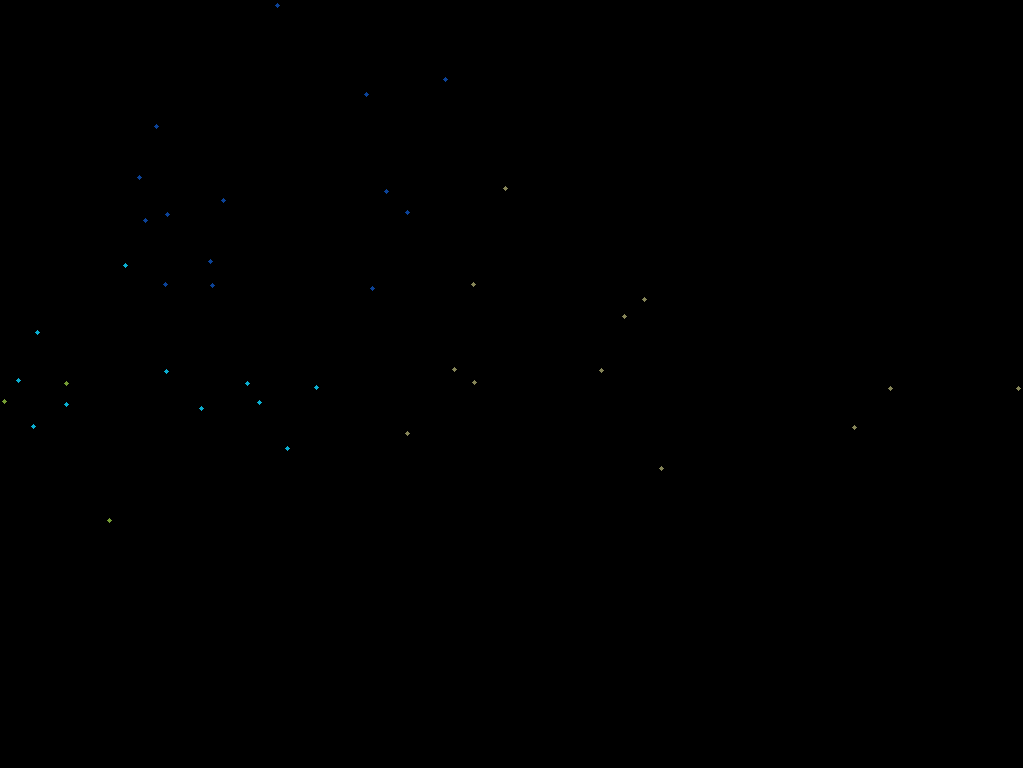
\includegraphics[width=0.8\textwidth]{ACP_SIFT.png} 
    \end{figure}
\begin{flushleft}
\begin{minipage}[t]{5cm}
Master 2 VIP, \\ Aurélien Cavelan et Jérôme Richard
\end{minipage}
\end{flushleft}

\end{titlepage}
%\clearpage
\tableofcontents

\chapter{Objectifs}

L'objectif de ce mini-projet consiste à développer un système de classification automatique non supervisée de photos. Le système dispose initialement de photos annotées en cinq classes, fournies par l'enseignant, et comportant quelques pièges. Chaque photo se rattache à une seule classe. À partir de cet ensemble de photos annotées, le système doit extraire des descripteurs et proposer une classification non supervisée des images (clustering).


\chapter{Choix Logiciels}

\section{Approche}
    Nous avons envisagé plusieurs outils pour réaliser ce projet, parmis lesquels :

    \begin{itemize}
        \item Matlab
        \item C++ - OpenCV
        \item Python - Scikit / Skimage
        \item Python - OpenCV
    \end{itemize}

    Matlab n'est pas assez performant et ne permet pas de répondre à tous nos besoins. Il n'est pas assez bas-niveaux et ne permet pas de développer un réel outil.

    Python est un langage très simple et il existe un kit de développement performant (binding C) disposant d'outils pour la classification, l'apprentissage et la manipulation d'images. Le manque de documentation et d'exemples nous a poussé à regarder du côté d'OpenCV.

    Le couple C++ OpenCV est probablement l'un des choix les plus courants pour la tâche qui nous est donnée. OpenCV est une bibliothèque très performante, bien qu'elle soit moins accessible que les options précédentes. On trouve néanmoins de nombreux exemples de codes utilisant OpenCV, et notamment pour lire des images, appliquer des filtres, extraire des descripteurs, ou encore utiliser l'algorithme des K-Moyennes ou la classification hiérarchique. C'est donc sur cette base que nous avons décidé de partir.

    Dans un premier temps, nous avons décidé d'implémenter un descripteur "moyenne de niveau de gris", car c'est un descripteur à une seule dimension et il est donc facile de vérifier les résultats de l'algorithme K-Moyennes. Nous avons également créé des jeux de données plus simples disponibles dans data2, data3 et data4 afin de comparer plus simplement les descripteurs. Par la suite nous avons implémenté d'autres descripteurs comme les Moments de Hu, Sift ou encore Surf, et nous avons utilisé différents paramètres ainsi que différentes méthodes de classification.


\section{Architecture}
    Le code est entièrement écrit en C++ et utilise la bibliothèque OpenCV. Un Makefile à la racine permet de compiler les différents algorithmes de classifications et les programmes se trouvent dans le dossier bin.

    Le programme prend en entrée un fichier .csv décrivant les images à utiliser et les classes auxquelles elles appartiennent. Le programme se sert d'une base d'images afin de déterminer les centres, soit par l'algorithme des K-Moyennes, soit par la classification hiérarchique (dendrogramme). Le programme classifie ensuite la totalité des images et affiche les résultats en mode texte, ainsi que l'indice de Rand et l'ACP sur deux dimensions.

    Le code du programme est peut fonctionner avec n'importe quel type de descripteurs et se trouve dans le fichier src/main.cpp. Les descripteurs implémentés se trouvent dans le fichier src/descriptors.cpp. Un descripteur est défini comme étant un ensemble de nombres flottants, typiquement 1 pour le descripteur "moyenne de niveau de gris" et 128 pour le descripteur "SURF".

    La répartition des images est également affichée lors de l'exécution du programme. Il est aussi possible d'exporter la position des centres dans fichier.

    Un certain nombre de données sont sauvegardés au format yml lors de l'exécution, tels que les descripteurs de SURF et de SIFT ainsi que le dictionnaire (Bag of Words) associé. Ils peuvent ainsi être réutilisés par OpenCV pour éviter de recalculer l'ensemble des descripteurs, ce qui peut prendre plus d'une minute.

    Les algorithmes SIFT et SURF sont actuellement brevetés et ne sont pas entièrement libres de droits. OpenCV inclut une implémentation de ces algorithmes, mais celle-ci est fournie dans le module \textit{nonfree} qui n'est pas présent sous Ubuntu par défaut (mais qui reste disponible sur les autres distributions). Nous avons donc récupéré le code source de ces algorithmes sur le dépôt d'OpenCV et nous les compilons séparément dans notre projet.


\section{Validation croisée}
    Notre programme est découpé en trois parties. La première partie consiste à extraire les descripteurs des images, au moyen d'une fonction externe (implémentée dans descriptors.cpp).

    Nous choisissons ensuite des images aléatoirement, par exemple 10 sur 50 que nous allons séparer en cinq classes à l'aide d'un dendrogramme ou de kmeans. Les cinq centres obtenus sont sauvegardés.

    Nous prenons ensuite les descripteurs de toutes les images restantes et nous les associons ou centre le plus proche afin de répartir toutes les images dans les cinq classes. La qualité de la distribution est mesurée avec l'indice de Rand. Nous répétons cette opération plusieurs fois jusqu'à obtenir les cinq centres qui donnent les meilleurs résultats.


\chapter{Descripteurs}
    Nous avons implémenté plusieurs descripteurs, certains très simples (et peu efficaces), et d'autres plus complexes mais aussi plus performants. Nous avons comparé ces descripteurs selon plusieurs critères, en comparant les résultats obtenus avec l'algorithme des K-Moyennes et la classification hiérarchique, mais aussi leur résistance à diverses transformations ou encore leur performance.

    \section{Descripturs 1D}
        Nous avons implémenté des descripteurs à une seule dimension très simples, principalement pour tester la validité de notre code et pour avoir un indice de référence. Comme nous nous y attendions, la classification est médiocre. Nous nous sommes également intéressé au filtre de Gabor, mais celui-ci n'est pas adapté aux images complexes et son utilisé réside principalement dans l'analyse de textures.

    \section{Moments de Hu}

        Les moments de Hu sont l'un des premiers déscripteurs avancés que nous avons utilisés. Nous nous sommes dit que l'analyse des formes présentes dans les images pourrait permettre ensuite de créer des descripteurs efficaces afin d'obtenir une bonne classification. En effet, on peut voir que les images du jeu de données mis à disposition contiennent des éléments distinguables par leur forme notamment les buildings (rectangles) et les pyramides (triangles), bicycles (cercles). Nous avons eu quelques difficultés à faire de la classification avec les descripteurs générés par les moments de Hu car cet algorithme génère plusieurs descripteurs par image. Chaque descripteur est alors associé à des formes détectées dans l'image. Notre idée a été de classifier tous les descripteurs de toutes les images et d'associer une classe à chacune. Le sens des classes pourrait ainsi être "être un carré" ou "être un cercle". Ensuite, pour chaque image, on regarde quelle classe est dominante dans tous ses descripteurs et on lui affecte cette classe. Une image contenant alors plein de triangle et peu de carrés est classée comme contenant des triangles.

        Bien que l'idée nous semblait prometteuse, les premiers résultats n'étaient pas très encourageants et cela était le reflet de multiples problèmes. En effet, nous avons constaté que la détection de contours qui précède les moments de Hu ne donne pas de très bons résultats (algorithme Canny précédé d'un flou gaussien). Il est donc difficile pour les moments de Hu de générer de bons descripteurs à partir de résultats difficilement exploitables. Afin de voir ce qui se passe lorsque le filtre de Canny donne de bons résultats, nous avons mis au point un autre jeu de données contenant des images avec des cercles des rectangles et des étoiles à classer en 3 catégories et les résultats étaient radicalement différents. En effet, l'ACP nous montre que cela donne 3 groupes de points très denses dans chaque groupe. Sur un autre jeu de données, contenant des images avec des cercles et des carrées de tailles différentes (2 classes), les résultats montraient globalement deux classes mais elles étaient difficiles à discerner, car bien que les données soient pratiquement linéairement séparables, la densité des deux groupes de points formés est très hétérogène et la classification en utilisant l'algorithme Kmeans ne pouvait pas donner des résultats satisfaisants.

        On peut donc dire que les moments de Hu ne sont pas bien adaptés au problème car les images traitées sont complexes induisant une mauvaise détection de contours et les descripteurs générés par l'algorithme ne sont pas directement viables pour être utilisé avec Kmeans ou même un dendrogramme. Nous pensons que si l'apprentissage avait été supervisé et avec un jeu de données plus simple, l'utilisation d'un SVM comme classifieur des descripteurs d'images générés par les moments de Hu aurait donné des résultats prometteurs.

    \section{SIFT / SURF}
        SIFT et SURF sont deux techniques qui permettent d'extraire des points-clés (local features) d'une image. Ces points-clés ne sont pas utilisables tel quel, et il peut y en avoir un grand nombre pour une seule image. 

        Le principe consiste à se servir de ces points pour constituer un dictionnaire de mots visuels. On commence par choisir des images pour lesquelles on extrait des points-clés (bag of words). À l'aide d'un algorithme de clustering comme kmeans, on va ensuite extraire les points les plus représentatifS (centres) parmi tous les points obtenus afin de créer un dictionnaire. Comme cette procédure peut prendre du temps (1 à 2 minutes pour SIFT, 30 secondes pour SURF), on enregistre le dictionnaire dans un fichier au format yml. Si ce fichier existe, notre programme va directement charger le dictionnaire existant pour effectuer la classification.

        Grâce au dictionnaire, on peut maintenant calculer pour chaque image un histogramme qui correspond à la distribution des mots du dictionnaire pour cette image (ensemble de nombre flottants entre 0 et 1). On peut aussi voir cet histogramme comme la contribution de chaque \textit{mot} du dictionnaire dans la description de l'image. Plus un \textit{mot} est apte à décrire l'image, plus la valeur qui lui est associée est élévée. L'histogramme est normalisé et peut donc être utilisé comme descripteur.


\chapter{Résultats}

\section{Comparaisons}
  Ci-dessous les mesure de l'indice de Rand obtenu avec différents descripteurs et paramètres sur les 50 images fournies. Ces images sont difficiles mais SIFT et SURF permettent d'obtenir d'assez bons résultats. Il n'est pas rare qu'une image soit assez différente de toutes les autres et que kmeans en fassent une seule classe (ne laissant que quatre classes pour les autres images). De plus, on peut parfois comprendre la cause d'une erreur, comme un bateau pouvant être facilement confondu avec une piramide à cause de ses lignes et de ses angles.

  \begin{figure}[!h]
      \centering
        \begin{tabular}{ | l | c | l | l |}
          \hline
          Descripteurs & Pré-traitement & Algorithme & Rand \\
          \hline
            Moyenne & -             & kmeans/hiérarchique   & 0.65\\
            Gabor   & -             & kmeans/hiérarchique   & 0.67\\
            SURF    & blur + canny  & kmeans/hiérarchique   & 0.66\\
            SIFT    & blur + canny  & kmeans/hiérarchique   & 0.68\\
            SURF    & -             & kmeans                & 0.70\\
            SIFT    & -             & kmeans                & 0.75\\
            SURF    & -             & hiérarchique          & 0.72\\
            SIFT    & -             & hiérarchique          & 0.78\\
          \hline  
        \end{tabular}
    \caption{Mesure de l'indexe de Rand sur les 50 images fournies}
  \end{figure}

  Afin de pouvoir distinguer les algorithmes de manière plus claire, nous avons créé deux jeux de données. Le premier est constitué de formes simples comme des cercles, des rectangles et des étoiles, avec des translations et des rotations. Sur ce jeu de donnée, on remarque que SIFT et SURF obtiennent d'excellents résultats, mais la moyenne également car la forme est simple et se trouve sur un fond unicolor. Nous avons donc créé un jeu de donner réel composé d'images de chiens et de roses. Les résultats sont parlants, SIFT et SURF obtiennent une classification presque parfaite, tandis que les autres techniques que nous avons vus ne donnent aucun résultat.

  \textbf{Note : } les images se trouvent dans les dossiers data.

  \begin{figure}[!h]
      \centering
        \begin{tabular}{ | l | c | l | l |}
          \hline
          Descripteurs & Pré-traitement & Algorithme & Rand\\
          \hline
            Moyenne & -             & hiérarchique          & 0.57\\
            Gabor   & -             & hiérarchique          & 0.52\\
            SURF    & -             & hiérarchique          & 0.88\\
            SIFT    & -             & hiérarchique          & 1.00\\
          \hline  
        \end{tabular}
    \caption{Mesure de l'indexe de Rand sur les 50 images fournies}
  \end{figure}

  
\end{document}

    
